\documentclass[12pt]{article}
\usepackage{tikz}
\usepackage[margin=1in]{geometry}
\usepackage{xcolor}
\usepackage{fontspec}

\usetikzlibrary{shapes,arrows,positioning,calc,fit}

\begin{document}

\begin{figure}[htbp]
\centering
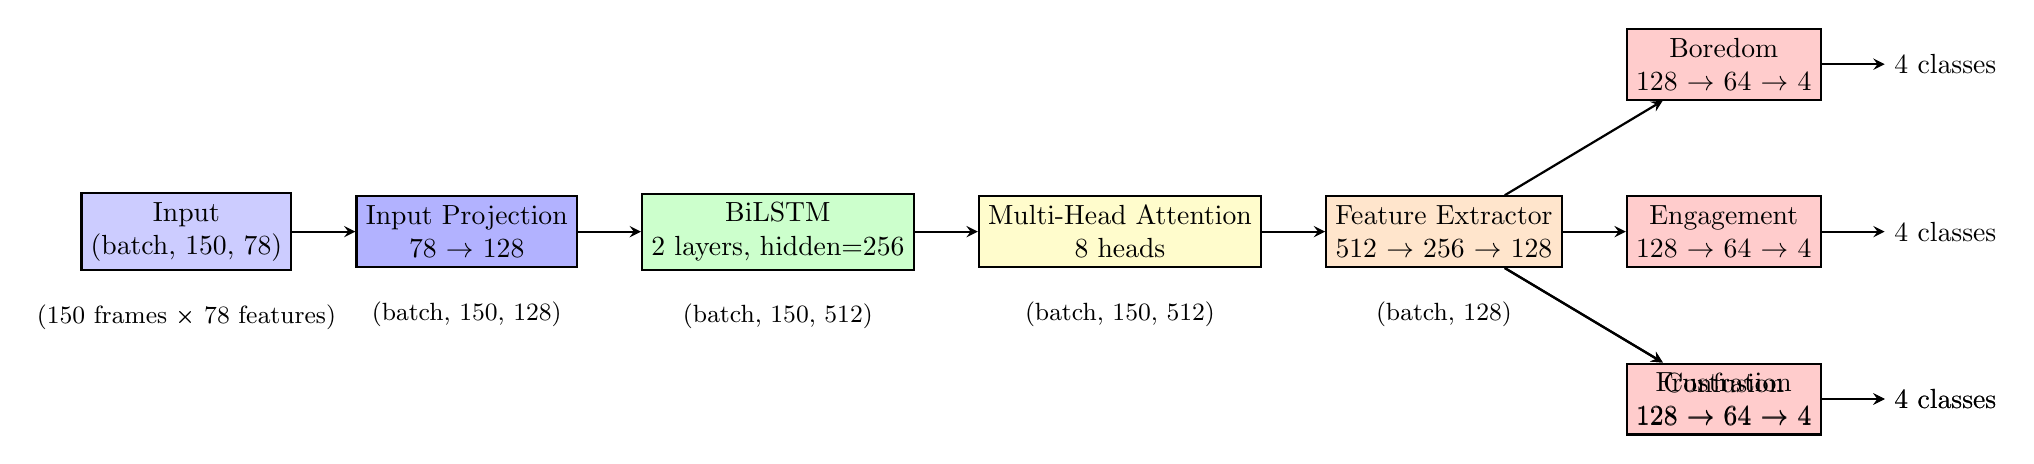
\begin{tikzpicture}[
    node distance=12mm and 8mm,
    box/.style={rectangle, draw, thick, align=center, minimum height=8mm},
    arrow/.style={->, thick, >=stealth},
    label/.style={text width=2.5cm, align=center, font=\small}
]

% Input Layer
\node[box, fill=blue!20] (input) {Input \\ (batch, 150, 78)};

% Input Projection
\node[box, fill=blue!30, right=of input] (proj) {Input Projection \\ 78 $\rightarrow$ 128};

% LSTM
\node[box, fill=green!20, right=of proj] (lstm) {BiLSTM \\ 2 layers, hidden=256};

% Attention
\node[box, fill=yellow!20, right=of lstm] (attn) {Multi-Head Attention \\ 8 heads};

% Feature Extraction
\node[box, fill=orange!20, right=of attn] (feat) {Feature Extractor \\ 512 $\rightarrow$ 256 $\rightarrow$ 128};

% Task Heads
\node[box, fill=red!20, above right=of feat] (bore) {Boredom \\ 128 $\rightarrow$ 64 $\rightarrow$ 4};
\node[box, fill=red!20, right=of feat] (enga) {Engagement \\ 128 $\rightarrow$ 64 $\rightarrow$ 4};
\node[box, fill=red!20, below right=of feat] (conf) {Confusion \\ 128 $\rightarrow$ 64 $\rightarrow$ 4};
 fill=red!20\node[box,, below=of enga] (frus) {Frustration \\ 128 $\rightarrow$ 64 $\rightarrow$ 4};

% Output labels
\node[right=of bore] (out1) {4 classes};
\node[right=of enga] (out2) {4 classes};
\node[right=of conf] (out3) {4 classes};
\node[right=of frus] (out4) {4 classes};

% Arrows
\draw[arrow] (input) -- (proj);
\draw[arrow] (proj) -- (lstm);
\draw[arrow] (lstm) -- (attn);
\draw[arrow] (attn) -- (feat);
\draw[arrow] (feat) -- (bore);
\draw[arrow] (feat) -- (enga);
\draw[arrow] (feat) -- (conf);
\draw[arrow] (feat) -- (frus);
\draw[arrow] (bore) -- (out1);
\draw[arrow] (enga) -- (out2);
\draw[arrow] (conf) -- (out3);
\draw[arrow] (frus) -- (out4);

% Dimension annotations
\node[below=0.3cm of input, font=\small] {(150 frames × 78 features)};
\node[below=0.3cm of proj, font=\small] {(batch, 150, 128)};
\node[below=0.3cm of lstm, font=\small] {(batch, 150, 512)};
\node[below=0.3cm of attn, font=\small] {(batch, 150, 512)};
\node[below=0.3cm of feat, font=\small] {(batch, 128)};

\end{tikzpicture}
\caption{LSTM Model Architecture for Multi-Task Affective State Recognition}
\end{figure}

\end{document}
